\chapter{The CMS Detector}
\label{sec:cms}

The Compact Muon Solenoid (CMS) detector is one of two hermetic, general purpose detectors at the Large Hadron Collider.
The original motivation for the experiment was the discovery of the Higgs boson by observing its decays to photons, electrons, and muons.
Towards this end, the detector was built to fulfill the following goals:
\begin{itemize}
\item Unambiguous charge identification of muons with momenta up to 1\TeV
\item 1\GeV mass resolution on 100\GeV pairs of muons, electrons, and photons
\item Efficient triggering and tagging of $\tau$ lepton and $b$ quark decays
\item Good resolution on the hadronic energy and missing transverse energy
\item Sufficient time resolution to deal with 40 MHz of collisions
\end{itemize}
The CMS detector consists of four main subdetetors: the inner tracker system, the electromagnetic calorimeter (ECAL), the hadronic calorimeter (HCAL), and the muon chambers.
The first three are within the field volume of the eponymous 3.8 T superconducting NbTi solenoid magnet while the muon chambers are embedded in the return yoke of the magnet.
Additionally, there is an online triggering system to reduce readout from 40 MHz to $\mathcal{O}(1)$ kHz for prompt reconstruction. 

\begin{figure}[htbp]
  \centering
  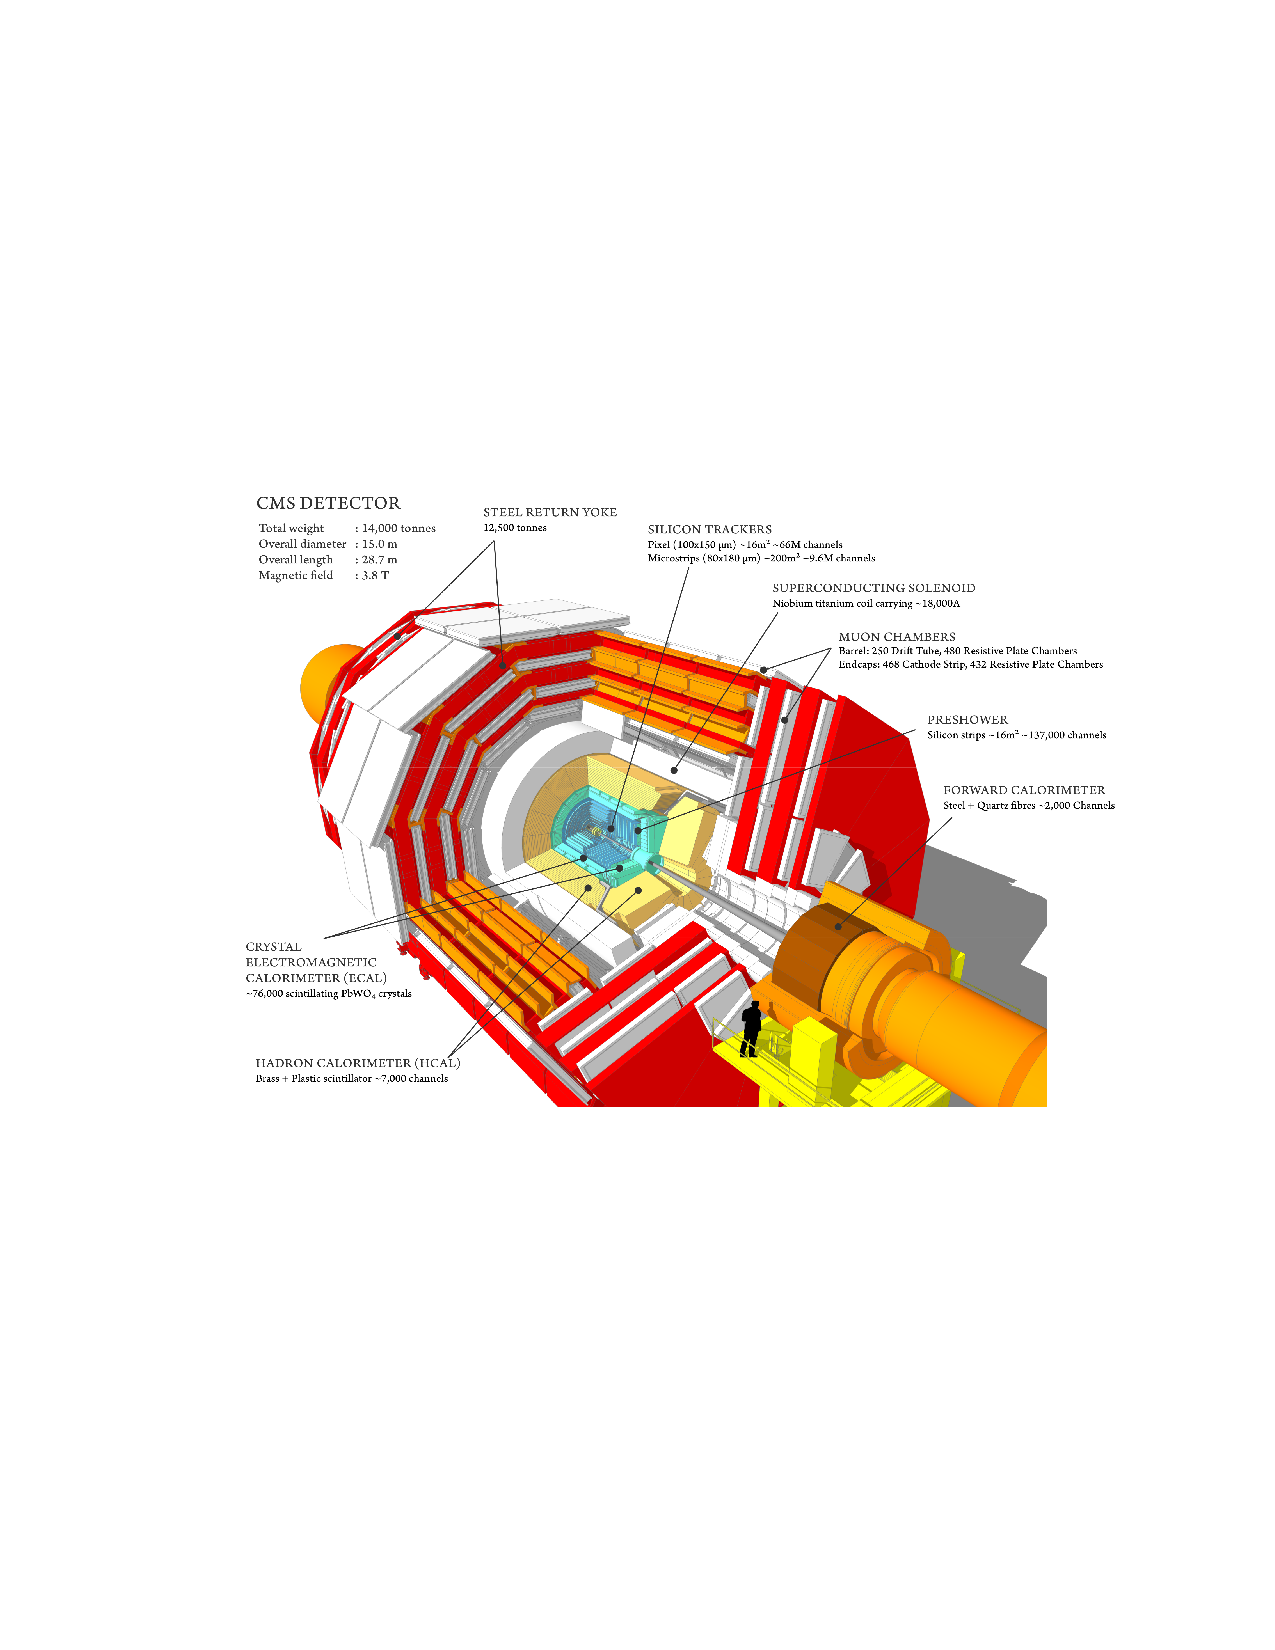
\includegraphics[width=0.9\textwidth]{Detector/Figures/cms_detector.pdf}
  \caption{
    A cutaway view of the CMS detector.
    The labels identify the solenoid as well as the different subdetectors and their components. 
    Reprinted from Reference~\cite{}. % http://cms.web.cern.ch/news/cms-detector-design
  }
  \label{fig:cms}
\end{figure}

The overall layout of the CMS detector is shown in Figure~\ref{fig:cms}. 
The CMS detector has a weight of 12500 tons, a length of 22 m, a diameter of 15 m, and a cylindrical geometry with concentric barrel shaped detectors in the central region and disc shaped detectors in the forward region.
The following coordinate system is used when working with the CMS detector:
\begin{itemize}
\item distance $z$ along the beam axis
  \begin{itemize}
  \item $z=0$ at the center of the detector
  \item positive corresponds to counter-clockwise as seen from the sky
  \end{itemize}
\item distance $r$ from the beam axis
\item polar angle $\theta$ measured with respects to the positive $z$-axis
\item azimuthal angle $\phi$ in the plane orthogonal to the beam axis
\end{itemize}
In addition to these four main coordinates, we define the right-handed cartesian $x$ and $y$ coordinates perpendicular to the beam axis, with the positive $x$-axis pointing from the center of the detector to the center of the LHC ring and the positive $y$-axis pointing upwards.

The four-momentum of a particle is $p = (p_x, p_y, p_z, E)$ in the cartesian basis 
%, where the first three components are space-like and the last one is time-like,
and a particle of mass $m$ produced at rest in the center of the detector has $p = (0, 0, 0, m)$.
While the momenta along the beam axis of the two incoming protons are equal, the momenta of the incoming partons involved in the hard scattering often are not as discussed in Section~\ref{sec:collider_pheno}.
Thus, we define two kinematic quantities that are Lorentz-invariant with respect to a boost along the beam axis:
the tranverse momentum $\ptvec = p_x \hat x + p_y \hat y$ with magnitude $\pt = \sqrt{p_x^2 + p_y^2}$ and the pseudorapidity $\eta = - \ln \tan\sfrac{\theta}{2}$.

In terms of \pt, $\eta$, and $\phi$, we have the following expressions for our cartesian variables: $p_x = \pt \cos \phi$, $p_y = \pt \sin \phi$, $p_z = \pt \sinh \eta$, and $E = \pt \cosh \eta$, with the last equality assuming the mass of the particle is negligible compared to its momentum.
In terms of our Lorentz-invariant coordinates, the four-momentum of a given particle is $p = (\pt, \eta, \phi, E)$. 
Additionally, the spatial separation of two particles is given by $\Delta R = \sqrt{(\Delta\phi)^2 + (\Delta\eta)^2}$ and the fiducial acceptance of the CMS detector is from $0 \le \phi < 2\pi$ and $-5 \le \eta \le 5$.

\section{Inner Tracker System}
\label{sec:cms_tracker}

Closest to the interaction point, the inner tracker system identifies charged particles and measures their momenta.
Additionally, high resolution tracks are used to identify primary and secondary vertices.
The magnetic field in the tracker volume is uniform with strength 3.8 T and field lines parallel to the beam direction. 
The tracker volume extends to 1.2 m in $r$ and 2.9 m in $z$, providing coverage for $\abs\eta < 2.5$,  and is instrumented with silicon pixels and strips.
Each silicon sensor is a $p$-$n$ semiconductor junction with a bias voltage applied.
When a charged particle passes through the depletion region of the junction, electron-hole pairs are produced and collected by the readout electronics.
A schematic of the inner tracker system is shown in Figure~\ref{fig:cms_tracker}.

\begin{figure}[htbp]
  \centering
  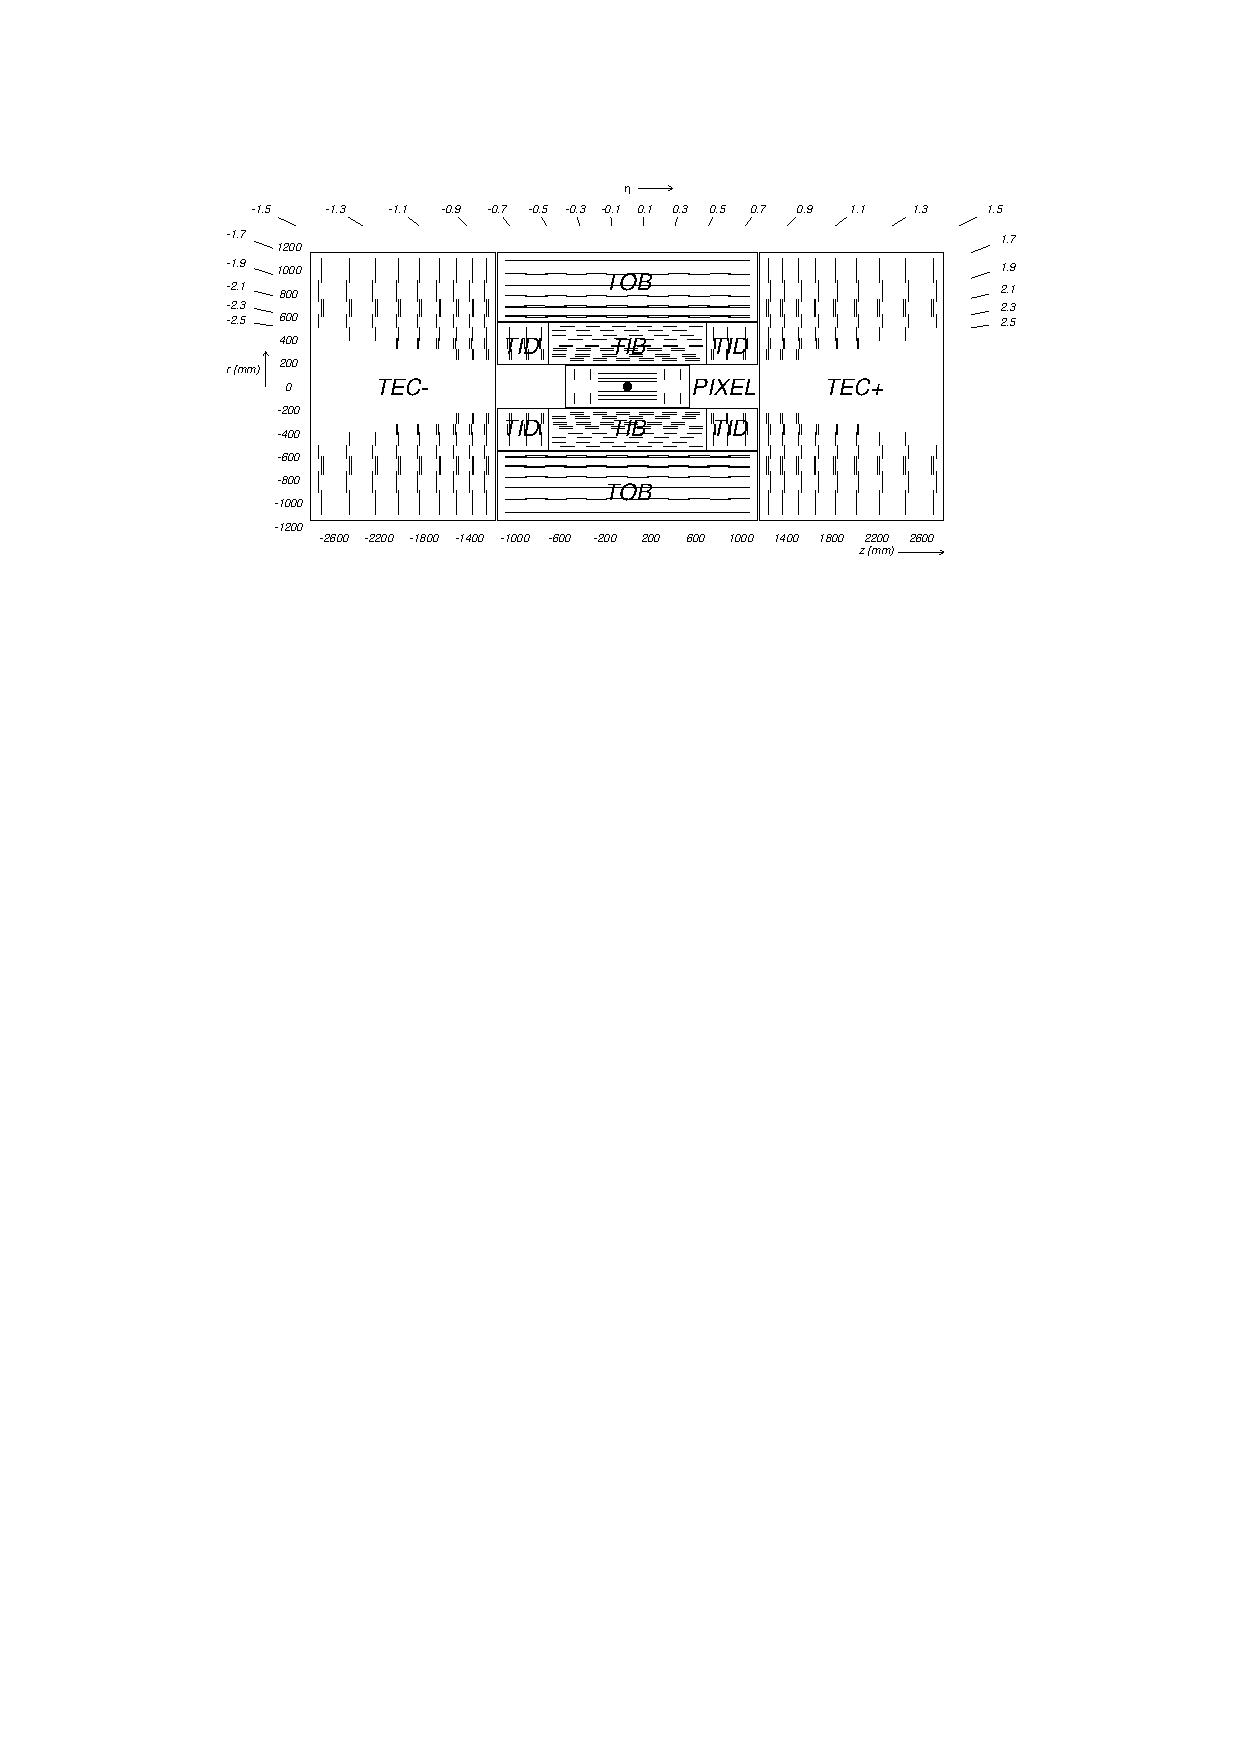
\includegraphics[width=\textwidth]{Detector/Figures/cms_tracker.pdf}
  \caption{
    A schematic view of the CMS inner tracker system.
    Silicon pixel and strip detectors are shown.
    The volumes labeled TIB, TID, TOB, and TEC are all strip trackers.
    The double lines indicate back-to-back modules that deliver stereo hits.
    % TIB = Tracker Inner Barrel, TID = Tracker Inner Disk, TOB = Tracker Outer Barrel, TEC = Tracker Endcap. 
    Reprinted from Reference~\cite{}. % https://iopscience.iop.org/article/10.1088/1748-0221/3/08/S08004/meta
  }
  \label{fig:cms_tracker}
\end{figure}

The 66 million individual pixel sensors, each measuring $285\mum\times 100\mum\times 150\mum$ in $r\times r\phi \times z$, are arranged into seven layers: three cylindrical barrels at $r = 4.4, 7.3, 10.2\cm$ and two bi-layer endcap annulli at $z = \pm34.5, \pm46.5 \cm$.
Due to the geometry of the pixel detector, tracks typically cross the sensor at a 20$^\circ$ angle, leading to the charge deposit from a single track to be shared among multiple pixels in the same layer.
The exact position of a particle in each layer is determined by interpolating the signals from multiple adjacent pixels with an analog pulse height greater than a tuneable read-out threshold.
Thus, each pixel hit is localized to an area of $\sim 15 \mum\times 20\mum$ in $r\phi \times z$, providing a much higher spacial resolution than the raw pixel spacing.

The pixels are surrounded 9.3 million silicon strips measuring $10\cm\times 80\mum$ arranged in ten cylindrical layers in the barrel and twelve disks in each endcap.
The Tracker Inner Barrel (TIB) consists of the first four layers and extends from 20\cm to 55\cm in the radial direction while out six layers constitute the Tracker Outer Barrel (TOB) with an outer radius of 116\cm and extent in $\abs z$ of 118\cm.
The remaining area in the barel is covered by the Tracker Inner Disk (TID), consisting of the three disks located from 80 to 90\cm in $\abs z$.
The Tracker EndCaps (TEC) have nine disks each and cover the region $124\cm < \abs z < 282\cm$.

The majority of the strips are oriented perpendicular to the $\phi$ direction: parallel to the beam pipe in the barrel region and radially aligned in the endcap region.
The strip pitch varies from 80 to 184\mum with the smallest pitch in the innermost layer.
This detector geometry provides good resolution in the $r$-$\phi$ plane for barrel and the $z$-$\phi$ plane for the endcap but little information on the orthogonal directions.
To compensate for this, one third of the strips are double-layered with a stereo angle of 100 mrad between the layers.
Matching hits between adjacent layers enables a measurement of the $z$ and $r$ coordinates in the barrel and endcap, respectively.
The final spacial resolution is 10-50\mum in the direction perpendicular to the strips and 100-530\mum in the parallel direction on the stereo modules.

% potential paragraph on tracker thickness

\section{Electromagnetic Calorimeter}

The electromagnetic calorimeter (ECAL) is a homogeneous, hermetic calorimeter
composed of 76,000 lead tungstate (PbWO4) crystals.
High density (8.3 g/$\cm^3$) lead tungstate was chosen due to its radiation hardnes, fast scintillation decay time constant of 25\ns, small Moliere radius $r_M= 21.9\mm$, and short radiation length $X_0 = 8.9\mm$.

The central barrel region (EB) has 61200 crystals arranged in a $170\times360$ $\eta$-$\phi$ grid with a coverage up to $\abs\eta = 1.44$ while the two endcap annuli (EE) each have 7324 crystals organized in a $x$-$y$ grid with coverage in the range $1.479 < \abs\eta < 3.0$.
Each crystal in the EB has a truncated pyramidal shape with a length of 230\mm, a $22\mm \times 22\mm$ front-face cross-section, and a $26\mm \times 26\mm$ rear-face cross-section while a crystal in the EE has a cuboid-like shape with a length of 230\mm, a $28.6 \mm \times 28.6\mm$ front-face cross-section, and a $30\mm \times 30\mm$ rear-face cross-section. 

\section{Hadronic Calorimeter}

Our big brassy boi.

\section{Muon Chambers}

The red ones.

\section{Online Trigger System}

How we choose events.

\section{Detector Simulation}

Gotta get predictions somehow.

% \section{Detector Issues}

% What went wrong.

